\documentclass[a4, 12pt]{scrreprt}

\usepackage{amsmath}
\usepackage[T1]{fontenc}
\usepackage[utf8]{inputenc}
\usepackage{enumitem}
\setlist[itemize]{nosep,after=\vskip-\baselineskip,leftmargin=*,before=\minipagetrue,}

\makeatletter
\newcommand{\minipagetrue}{\@minipagetrue}

\makeatother
\usepackage{graphicx}
\usepackage[T1]{fontenc}
\usepackage[ngerman]{babel}
\usepackage[colorlinks,
pdfpagelabels,
pdfstartview = FitH,
bookmarksopen = true,
bookmarksnumbered = true,
linkcolor = black,
plainpages = false,
hypertexnames = false,
citecolor = black] {hyperref}

\setkomafont{section}{\fontsize{12}{13}}
\setcounter{secnumdepth}{3}
\setcounter{tocdepth}{3}

\begin{document}
\tableofcontents

\let\cleardoublepage\clearpage
\chapter{wichtige Minerale}

\begin{tabular}{p{5cm}@{}|p{12,2cm}@{}}
Mineral & Infos\\
\hline

\section{Quarz} & 
\begin{tabular}{p{3cm}@{}p{9cm}@{}}
Formel & $SiO_2$\\
Ausbildung & oft in Drusen/grobkörnig, säulig mit 6-eckigem Querschnitt und Dachflächen, oft xenomorph\\
Bruch & keine Spaltbarkeit $\rightarrow$ muscheliger Bruch\\
Glanz & auf Bruchflächen Fettglanz, Kristallflächen Glasglanz\\
Farbe & Im Gestein oft farblos bis grau-glasig\\
Härte & 7\\
Dichte & 2,65 $\frac{g}{ch^3}$\\
Vorkommen & zweithäufigstes Mineral in der Erdkruste, nur in ultramarphischen Gesteinen abwesend\\
Varietäten & 
\begin{itemize}
\item Amethyst (violett)
\item Rauchquarz (gelb/braun, schwarz)
\item Citrin (gelblich)
\item Milchquarz (weiß)
\item Rosenquarz (rosa)
\item Bergkristall (transparent)
\end{itemize}\\
\end{tabular}\\
\hline

\section{Feldspatgruppe:}\\
 & 
\begin{tabular}{p{3cm}@{}p{9cm}@{}}
Kristallsystem & monoklin/triklin\\
Ausbildung & selten idiomorph, isometrische/tafelige/ prismatische Form\\
Zwillinge & 
\begin{tabular}{p{3cm}@{}|p{6cm}@{}}
Alkalifeldspat & Karlsbader\\
Plagioklas & polysynthetische Zwillinge\\
\end{tabular}\\

Bruch & 2 gute spaltbarkeiten, 1 schlechte\\
Farbe & 
\begin{tabular}{p{3cm}@{}|p{6cm}@{}}
Alkalifeldspat & weiß, oft fleischfarbend, auch ziegelrot\\
Plagioklas & weiß-grau, häufig mit grünem Stich\\
\end{tabular}\\
Glanz & Glasglanz/Perlmuttglanz\\
Transparenz & Plagioklas Mikroklin und Orthoklas durchsichtig\\
 & Sanidin glasig\\
Härte & 6\\
Dichte & 2,6 bis 2,8$\frac{g}{ch^3}$\\
Vorkommen & häufigstes Mineral in der Erdkruste\\
\end{tabular}\\

Kalifeldspat (Orthoklas) &
\begin{tabular}{p{3cm}@{}p{9cm}@{}}
\hline
Formel & $K [AlSi_3O_8]$\\
\end{tabular}\\


Natriumfeldspat (Albit) &
\begin{tabular}{p{3cm}@{}p{9cm}@{}}
Formel & $Na [AlSi_3O_8]$\\
\end{tabular}\\


Calciumfeldspat &
\begin{tabular}{p{3cm}@{}p{9cm}@{}}
Formel & $Ca [AlSi_3O_8]$\\
\end{tabular}\\
(Anorithit)\\
\hline

\end{tabular}
\newpage



\begin{tabular}{p{3cm}@{}|p{12,2cm}@{}}
\hline

\section{Biotit} & 
\begin{tabular}{p{3cm}@{}p{9cm}@{}}
Kristallsystem & monoklin, pseudohexagonal\\
Ausbildung & oft tafelige, pseudohexagonale Kristalle, blättrig bis schuppig\\
Bruch & 1 ausgezeichnete Spaltbarkeit, elastisch\\
Farbe & braun bis schwarz, selten grünlich\\
Glanz & auf frischen Spaltflächen Metallglanz/lackig\\
Härte & 2,5 bis 3\\
Dichte & ca. 3 $\frac{g}{cm^3}$\\
Vorkommen & 
\begin{tabular}{p{3cm}@{}p{6cm}@{}}
magmatisch & Diorit, Tonalit, Granodiorit, Granit, Dazit, Rhyolith\\
metamorph & u.a. in Phyllit, Schiefer, Gneis\\
\end{tabular}
\end{tabular}\\
\hline

\section{Muskovit} & 
\begin{tabular}{p{3cm}@{}p{9cm}@{}}
Kristallsystem & monoklin/pseudohexagonal\\
Ausbildung & tafelige pseudohexagonale Kristalle, blättrig bis schuppig, selten feinkörnig\\
Bruch & 1 ausgezeichnete Spaltbarkeit (bättrig)\\
Farbe & überwiegend farblos/transparent, auch gelb- bis grünlich, beige\\
Glanz & Perlmuttartig/silberglänzend\\
Härte & 2,5 bis 3\\
Dichte & ca. 2,8 $\frac{g}{cm^3}$\\
Vorkommen & 
\begin{tabular}{p{3cm}|@{}p{5,5cm}@{}}
metamorph & Phyllit, Schiefer\\
magmatisch & Granit\\
pegmatisch & \\
\end{tabular}\\
\end{tabular}\\
\hline

\section{Amphibole} &
\begin{tabular}{p{3cm}@{}p{9cm}@{}}
Kristallsyst & 
\begin{tabular}{p{3cm}@{}p{6cm}@{}}
Orthoamphibole & orthorhombisch\\
Klinoamphibole & monoklin\\
\end{tabular}\\
Ausbildung & prismatische Kristalle mit 6-eckigem Querschnitt, oft auch nadelig oder faserig\\
Bruch & 2 gute Spaltbarkeiten (56°, 124°)\\
Glanz & nichtmetallisch, stärker als bei Pyroxen\\
Farbe & 
\begin{tabular}{p{3cm}|@{}p{5,5cm}@{}}
Hornblende & dunkelbraun/grün bis schwarz\\
Aktinolith & grün bis schwarzgrün\\
Tremolit & weiß\\
Riebeckit, & blau bis schwarzblau\\
Glaukophan\\
Anthopphyllit & grau\\
\end{tabular}\\
Härte & 5 bis 6\\
Dichte & 2,9 bis 3,2\\
Habitus & häufig prismatisch oder nadelig\\
Vorkommen & 
\begin{tabular}{p{3cm}|@{}p{5,5cm}@{}}
magmatisch & Hornblende, Riebeckit\\
metamorph & Hornblende Tremolit, Aktinolit, Anthophylit, Glaukophan, Roebeckit\\
\end{tabular}\\
\end{tabular}\\
\hline
\end{tabular}

\begin{tabular}{p{3cm}@{}|p{12,4cm}@{}}
\hline

\section{Pyroxene} &
\begin{tabular}{p{3cm}@{}p{9cm}@{}}
Kristallsystem & 
\begin{tabular}{p{3cm}@{} |p{5,5cm}@{}}
Orthopyroxene & orthorhombisch\\
Klinopyroxene & monoklin\\
\end{tabular}\\
Ausbildung & prismatische Kristalle mit quadratischem, meist 8-seitigem Querschnitt\\
Bruch & 2 gute Spaltbarkeiten-90°\\
Glanz & nichtmetallisch, matter als Amphibole\\
Farbe & 
\begin{tabular}{p{4cm}@{} |p{6cm}@{}}
Augit, Hypersthen, Orthoferrosilit & dunkelbraun bis schwarz\\
Diopsid bis Hedenbergit bis Augit Aegirin & grün bis schwarzgrün\\
Jadit bis Omphacit & weiß bis grün\\
\end{tabular}\\
Härte & 5 bis 6\\
Dichte & 3,1 bis 3,5\\
Habitus & langprismatisch bis stängelig\\
Vorkommen & 
\begin{tabular}{p{3cm}@{}|p{6cm}@{}}
magmatisch & Diopsid, Augit Orthopyroxen, Aegirin\\
metamorph & Diopsid-Hadenbegit, Orthopyroxene, Jadit-Omphacit, Aegirin\\
\end{tabular}\\
\end{tabular}\\
\hline

\section{Olivin} & 
\begin{tabular}{p{3cm}@{}p{9cm}@{}}
Kristallsystem & orthorhombisch\\
Ausbildung & meist körnig, selten gut ausgebildete Kristallflächen\\
Bruch & muschelig, 1 Spaltbarkeit\\
Glanz & Glasglanz, etwas fettig; transparent\\
Farbe & gelbgrün bis dunkelgrün, Mischkristalle i.d.R. flaschengrün, ockergelb bis bräunlich verwitternd\\
Härte & 7\\
Dichte & 3,3 bis 4,4\\
Vorkommen & in $SiO_2$ armen magmatiten und Metamorphiten; nicht in Paragenese mit Quarz\\
\end{tabular}\\
\hline

\section{Pyrit} & 
\begin{tabular}{p{3cm}@{}p{9cm}@{}}
Formel & $FeS_2$\\
Kristallsystem & Kubisch\\
Ausbildung & v.A. Würfel\\
Härte & 6 bis 6,5\\
Dichte 5 bis 5,2 $\frac{g}{cm^3}$\\
Spaltbarkeit & sehr undeutlich, meist muscheliger Bruch\\
Glanz & metallisch/opak\\
Farbe & messingartig bsi gold\\
Strichfarbe & schwarz mit leichtem grünstich\\
Vokommen & häufig in diversen gesteinen, jedoch mengenmäßig untergeordnet; Erzlagerstätten, Fossilisationsmaterial\\
\end{tabular}\\
\hline
\end{tabular}

\begin{tabular}{p{3cm}@{}|p{12,4cm}@{}}
\hline
\section{Spinell} & 
\begin{tabular}{p{3cm}@{}p{9cm}@{}}
Formel & 
\begin{tabular}{p{3cm}@{}p{6cm}@{}}
$MgAl_2O_4$ & 
\begin{itemize}
\item $Mg^{2+} \leftrightarrow Fe,Zn,Mn$
\item $Al^{3+} \leftrightarrow Fe,Mn,Cr$
\end{itemize}\\
\end{tabular}\\
Kristallsystem & kubisch \\
Ausbildung & oft oktaedrisch, verzwillingt\\
Härte & 7,5 bis 8\\
Dichte & 3,8 bis4,1 $\frac{g}{cm^3}$\\
Spaltbarkeit & keine, muscheliger Bruch\\
Glanz & meist Glasglanz\\
Farbe & bräunlich schwarz; selten rot, grün oder blau\\
Vorkommen & überwiegend metamorph\\
\end{tabular}\\
\hline

\section{Zirkon} & 
\begin{tabular}{p{3cm}@{}p{9cm}@{}}
Formel & $Zr[SiO_4]$\\
Kristallsystem & tetragonal\\
Ausbildung & oft oktaedrisch, häufig verzwillingt, oft körnig\\
Härte & 7,5\\
Dichte & 4,5 $\frac{g}{cm^3}$\\
Spaltbarkeit & keine, muscheliger Bruch\\
Glamz & meist Fettglanz, Diamantglanz\\
Farbe & bräunlich, selten gelb, grün oder farblos\\
Vorkommen & oft magmatisch (primär), seltener in Sedimenten angereichert
\end{tabular}\\
\hline 

\section{Leucit} & 
\begin{tabular}{p{3cm}@{}p{9cm}@{}}
Formel & $K[AlSi_2O_6]$\\
Kristallsystem & tetragonal, pseudokubisch\\
Ausbildung & ikositetraeda (24-Flächner) allg. rundliche Querschnitte\\
Bruch & keine Spaltbarkeit, muscheliger Bruch\\
Farbe & weiß bis grau\\
Härte &  5,5 bis 6\\
Dichte & 2,6 $\frac{g}{cm^3}$\\
Vorkommen & nur in (Sub-)Vulkaniten, tritt bei $SiO_2$-Untersättigung auf $\rightarrow$ nicht in Paragenese mit Quarz\\
\end{tabular}\\
\hline

\section{Nephelin} & 
\begin{tabular}{p{3cm}@{}p{9cm}@{}}
Formel & $Na[AlSiO_4]$\\
Kristallsystem & hexagonal\\
Ausbildung & in Vulkaniten oft gut mit rechteckigen bzw 6-eckigem Querschnitt, in Plutoniten oft xenomorph\\
Bruch & sehr unvollkommene SPaltbarkeit, muscheliger Bruch, rauer als Quarz\\
Farbe & transparent, weis oder grau grünlich, bräunlich, rötlich \\
Glanz & Glasglanz an den Spaltflächen, Fettglanz an Bruchflächen\\
Härte & 5 bis 6 (lässt sich im unterschied zu Quarz ritzen)\\
Dichte & ca2,6 $\frac{g}{cm^3}$\\
Vorkommen & magmatisch, vertritt Albit bei $SiO_2$-Untersättigung\\
\end{tabular}\\
\hline
\end{tabular}
\newpage

\begin{tabular}{p{3cm}@{}|p{12,4cm}@{}}
\hline
\section{Turmalin} &
\begin{tabular}{p{3cm}@{}p{9cm}@{}}
Formel & $NaFe_3^{2+}Al_6[Si_6O_{18}](BO_3)_3(OH)_4$\\
Kristallsystem & trigonal\\
Ausbildung & säulige Kristalle mit 3-eckigem Querschnitt, oft längsgestreift, häufig in radialstrahligen aggregaten\\
Bruch & keine Spaltbarkeit, jedoch Querbrüche der Säulen\\
Glanz & Glasglanz \\
Farbe & häufig schwarz, doch auch grün, blau, rot, braun, rosa, farblos,oft zonar\\
Härte & 7,5\\
Dichte & 2,9 bis 3,2 $\frac{g}{cm^3}$\\
Vorkommen & pegmatisch, magmatisch, metamorph\\
\end{tabular}\\
\hline

\section{Magnetit} &
\begin{tabular}{p{3cm}@{}p{9cm}@{}}
Formel & $Fe_3O_4$\\
Kristallsystem & kubisch\\
Ausbildung & xenomorphe Massen und Einzelkörner, idiomorphe Kristalle als Oktaeda vor Allem in Grünschiefern\\
Härte & 5,5\\
Dichte & 5,2 $\frac{g}{cm^3}$\\
Glanz & matter Metallglanz\\
Farbe & grauschwarz, schwarz\\
Srichfarbe & schwarz\\
Vorkommen & marphitreiche Magmatite, Erzlagerstätten, sedimentär als dentritische Komponente von Sanden\\
magnetisch & Ja\\
\end{tabular}\\
\hline

\section{Hämatit} &
\begin{tabular}{p{3cm}@{}p{9cm}@{}}
Formel & $Fe_2O_3$\\
Kristallsysthem & trigonal\\
Ausbildung & 3 Modifikationen: 
	\begin{tabular}{p{3cm}@{}|p{4,5cm}@{}}
	Eisenglanz & grobkristallin oder körnig-derb; stahlgrau\\
	Specularit \\
	(„Eisenglimmer“) & dünnblättrig-schuppige, glimmerartige Aggregate\\
	Roteisen & feinkristallin, oft faserig, z. T. auch locker erdig; tief braunrot bis rot\\
	\end{tabular}\\
Härte & 6,5 (wenn feinkörnig oft geringer)\\
Dichte & 5,2$\frac{g}{cm^3}$\\
Spaltbarkeit & keine aber 2 teilbarkeiten möglich\\
Glanz & matter Metallglanz, opak\\
Farbe & stahlgrau bis schwarz, rotbraun, bunt anlaufend, rot verwitternd\\
Strichfarbe & rot bis rotbraun\\
Vorkommen & häufig ein gleichmäßig oder fleckig fein-verteiltes rotes Pigment in verschiedensten Gesteinen\\
\end{tabular}\\
\hline
\end{tabular}

\newpage
\begin{tabular}{p{4cm}@{}|p{12,4cm}@{}}
\hline 
\section{Limonit} & 
	\begin{tabular}{p{3cm}@{}p{9cm}@{}}
	Farbe & SeO(OH)\\
	Kristallsysthem & Amorph\\
	Ausbildung & kann alles sein\\
	Härte & 5 bsi 5,5\\
	Dichte & 3,3 bis 4,3$\frac{g}{cm^3}$\\
	Glanz & von matt erdig bis hochglänzend\\
	Farbe & gelb bis braun\\
	Strichfarbe & gelbbraun\\
	Vorkommen & Bestandteil sedimentärer, eisenhaltiger Gesteine; in sekundären Lagerstätten\\
	\end{tabular}\\
\hline 

\section{Galenit (Bleiglanz)} & 
	\begin{tabular}{p{3cm}@{}p{9cm}@{}}
	Formel & PbS\\
	Kristallsystem & Kubisch\\
	Ausbildung & meist idiomorphe Kristalle, häufig gerundete Kanten; grobspätige Masse\\
	Härte & 2,5\\
	Dichte & 7,2 bis 7,6$\frac{g}{cm^3}$\\
	Spaltbarkeit & 3 sehr gute\\
	Glanz & intensiv-silbriger Metallglanz auf frischen flächen, opak\\
	Farbe & auf frischen Flächen silbriggrau, Außenflächen mattgrau; Anlaufflächen oft blau\\
	Strichfarbe & grauschwarz\\
	Vorkommen & ganz überwiegend in hydrothermalen Erzlagerstätten, seltener diagenetisch in Sedimentgesteinen\\
	\end{tabular}\\
\hline 

\section{Calcit} &
	\begin{tabular}{p{3cm}@{}p{9cm}@{}}
	Formel & $CaCO_3$\\
	Kristallsystem & trigonal\\
	Ausbildung & im Gesteinsverband immer xenomorph\\
	Härte & 3\\
	Dichte 2,7 bis 2,9$\frac{g}{cm^3}$\\
	Spaltbarkeit & 3 vollkommene Spaltbarkeiten\\
	Glanz & Glasglanz, Perlmuttglanz, auf Bruchflächen Perlmuttglanz\\
	Farbe & transparent (dann starke Doppelbrechung); milchig weiß, gelblich, rosa, grau, grün\\
	Vorkommen & Vorwiegend als Kalkstein; als hydrothermale Gangfüllung;
in magmatischen Karbonatiten; metamorph in Marmoren\\
	Reaktion mit HCl & reagiert sehr stark
	\end{tabular}\\
\hline
\end{tabular}

\newpage

\begin{tabular}{p{3cm}@{}|p{12,4cm}@{}}
\hline
\section{Gips} & 
	\begin{tabular}{p{3cm}@{}p{9cm}@{}}
	Formel & $CaSO_4 \cdot 2H_2O$\\
	Kristallsystem & monoklin\\
	Ausbildung & im Gestein xenomorph, idiomorphe Ausbildung in Hohlräumen und Tonen: dicktafeliger HJabitus mit Parallelogramm-förmigem Umriss\\
	Härte & 2\\
	Dichte 2,3$\frac{g}{cm^3}$\\
	Spaltbarkeit & 3 gute Spaltbarkeiten; häufig große Spaltflächen\\
	Glanz & Glasglanz, Perlmuttglanz oder Seidenglanz\\
	Farbe & weiß, grau, gelb, braun, bläulich; durchsichtig bis durchscheinend\\
	Vorkommen & massig-derb als Gipsgestein (Verwitterungsprodukt von Anhydritgestein aufgrund von Wasseraufnahme, (Volumenzunahme um ca. 60 \%); idiomorphe Gipskristalle in tonigen Sedimentgesteinen; an Austrittstellen vulkanischer Gase auf Ca-reichen Gesteinen; nie magmatisch oder metamorph\\
	\end{tabular}\\
\hline

\section{Anhydrit} &
	\begin{tabular}{p{3cm}@{}p{9cm}@{}}
	Formel & $CaSO_4$\\
	Kristallsystem & orthorhombisch\\
	Ausbildung & xenomorph \\
	Härte & 3 bis 3,5\\
	Dichte & 3$\frac{g}{cm^3}$\\
	Spaltbarkeit & 3 gute Spaltbarkeiten die sich je mit 90° schneiden\\
	Glanz & Perlmuttglanz, Glasglanz\\
	Farbe & weiß, farblos, hellblau, grau, rötlich, bräunlich; durchscheinend\\
	Vorkommen & als sedimentäres (diagenetisches) Anhydritgestein im Zusammenhang mit Salzlagerstätten; bildet sich primär als Ausscheidungsprodukt aus übersättigtem Meerwasser oder metamorph aus Gips durch Entwässerung\\
	\end{tabular}\\
\hline 

\section{Sylvin} & 
	\begin{tabular}{p{3cm}@{}p{9cm}@{}}
	Formel & KCl\\
	Kristallsystem & kubisch\\
	Ausbildung & idiomorphe Kristalle in Würfel- bzw. Oktaederform, körnig-massig\\
	Härte & 2,5\\
	Dichte & 2,2$\frac{g}{cm^3}$\\
	Spaltbarkeit & eine vollkommene Spaltbarkeit\\
	Glanz & Glasglanz\\
	Farbe & farblos bis weiß, hellgrau, hellblau, gelblich, rötlich, violett\\
	Vorkommen & in Evaporiten und als Sublimationsprodukt von Vulkanen\\
	weiteres & wasserlöslich, bitter im Nachgeschmack
	\end{tabular}\\
\hline
\end{tabular}

\newpage
\begin{tabular}{p{4cm}@{}|p{12,4cm}@{}}
\hline

\section{Baryt} & 
	\begin{tabular}{p{3cm}@{}p{9cm}@{}}
	Formel & $BaSO_4$\\
	Kristallsystem & orthorhombisch\\
	Ausbildung & meist grobspätig-derbe oder auch feinkörnig-dichte Massen bildend; fächerförmige Aggregate idiomorpher Kristalle\\
	Härte & 3 bis 3,5\\
	Dichte & 4,5$\frac{g}{cm^3}$\\
	Spaltbarkeit & 3 (sehr)gute Spaltbarkeiten\\
	Glanz & z.T. Glasglanz, Perlmuttglanz\\
	Farbe & zumeist milchig weiß, auch farblos transparent, gelblichgrau, grau, blassblau, rötlich braun\\
	Vorkommen & verbreitet als hydrothermales Mineral in Erzgängen; diagenetisch in Sedimentgesteinen als Bindemittel oder konkretionär; kein Gesteinsbestandteil in Magmatiten oder Metamorphiten\\
	\end{tabular}\\
\hline

\section{Halit (Steinsalz)} &
	\begin{tabular}{p{3cm}@{}p{9cm}@{}}
	Formel & NaCl\\
	Kristallsystem & kubisch\\
	Ausbildung & idiomorphe Kristalle in Würfelform, körnig-massig\\
	Härte & 2,5\\
	Dichte & 2,2$\frac{g}{cm^3}$\\
	Spaltbarkeit & 3 gute Spaltbarkeiten (schneiden sich bei 90°)\\
	Glanz & Glasglanz\\
	Farbe & transparent farblos-klar, rötlich getrübt, blaue Schlieren (selten)\\
	Vorkommen & wichtigstes Salzmineral; gesteinsbildend als ausschließliches oder nahezu ausschließliches Mineral des Gesteins Steinsalz; Ausfällungsprodukt bei der Eindampfung von Meerwasser und terrestrischen Salzseen; wegen hoher Wasserlöslichkeit nur in aridem Klima an der Erdoberfläche vorkommend; als Ausblühung in Steppen und Wüsten, am Rand von Salzseen, als Sublimationsprodukt von Vulkanen\\
	\end{tabular}\\
\hline 
\end{tabular}



\newpage
\chapter{die wichtigsten Minerale in Magmatiten}

\begin{tabular}{p{3cm}@{}|p{12cm}@{}}
felsische (helle) & 
\begin{itemize}
\item Quarz
\item Alkalifeldspat
\item Plagioklas
\item Foide
Feldspatvertreter (Foide)
\end{itemize}\\
maphische (dunkle) & 
\begin{itemize}
\item Glimmer: Biotit, Muskovit
\item Amphibole: meist Hornblende
\item Pyroxene
\item Olivin
\end{itemize}
\end{tabular}

\chapter{wichtige Minerale in Sedimentgesteinen}
\begin{itemize}
\item Quarz
\item Plagioklase, Feldspäte
\item Muskovit, Biotit, Tonminerale, Chlorit
\item Pyroxene, Amphibole
\item Calzit, Dolomit
\item Gips, Anhydrit, Steinsalz, Kalisalz
\item Pyrit
\end{itemize}

\chapter{Vergleich Plagioklas und Alkalifeldspat}

\begin{tabular}{l|p{7cm}@{}p{7cm}@{}}
Kriterium & Alkalifeldspat & Plagioklas\\
\hline
Spaltbarkeit & 90° zwischen den Spaltflächen & 86° Spaltwinkel\\
Farbe & farblos, weiß/rötlich & weiß-grünlich\\
Lamellen & Perthitlamellen (immer sichtbar) & polysynthetische Zwillingslamellen\\
Verzwillingung & Karlsbader & polysynthetische Zwillinge\\
Zonarbau & - & selten sichtbar\\
Verwitterug & meist frisch & verwittert leicht, hell, weiß, gelblich\\
\end{tabular}

\chapter{Vergleich Amphibol und Pyroxen}
\begin{tabular}{l|p{7cm}@{}p{7cm}@{}}
Kriterium & Amphibol & Pyroxen\\
\hline
Spaltwinkel & 60/120 & 90\\
Ausbildung der Spaltbarkeit & gut bis deutlich & weniger deutlich bis schlecht\\
Glanz & lackartig/glasglanz & matter als Amphibol\\
Habitus & langprismatisch bis stängelig & isometrisch bis prismatisch\\
\end{tabular}

\newpage
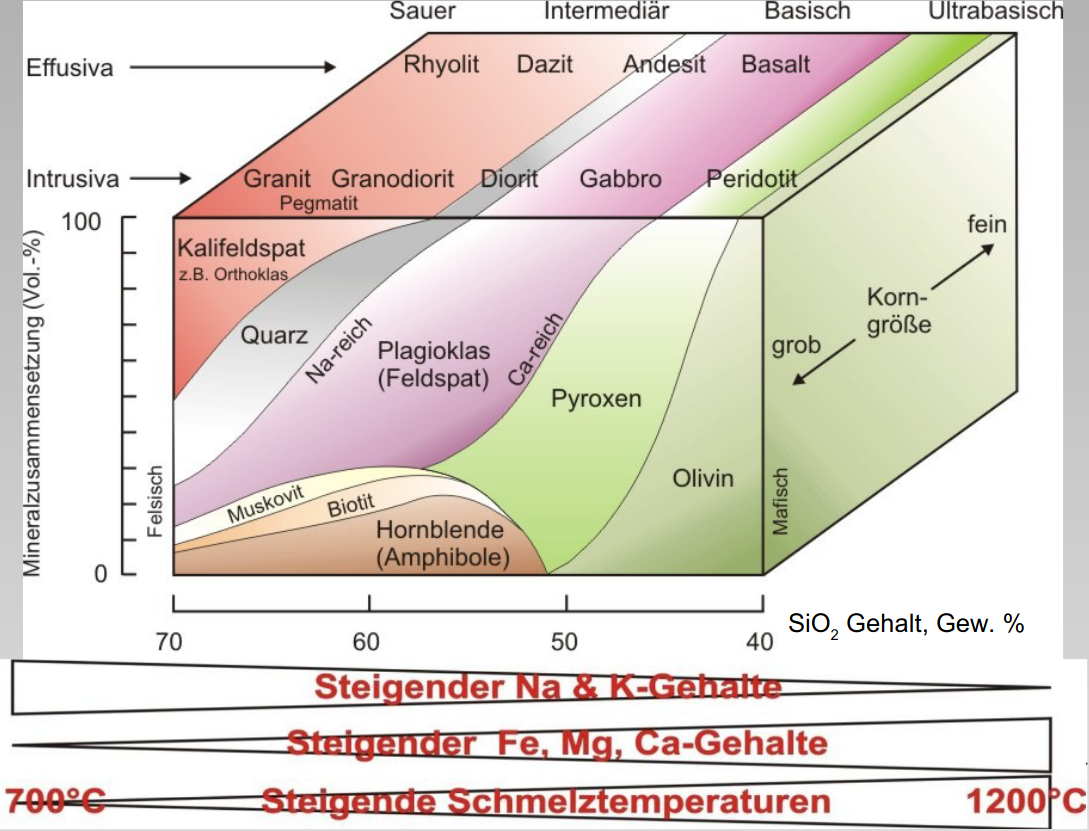
\includegraphics[width=0.8\textwidth]{/home/joni/Schreibtisch/Uni/Mittschriften/Bausteine Der Erde/Bilder/Silikatanteil}\\
\\
\includegraphics[width=0.8\textwidth]{/home/joni/Schreibtisch/Uni/Mittschriften/Bausteine Der Erde/Bilder/Feldspäte}

\end{document}